\documentclass[a4paper,10pt]{article}
\usepackage{fullpage}
\usepackage[british]{babel}
\usepackage[T1]{fontenc}
\usepackage{amsmath}
\usepackage{amssymb}
\usepackage[T1]{fontenc}
\usepackage[utf8]{inputenc}
%\usepackage{amsthm} \newtheorem{theorem}{Theorem}
\usepackage{color}
\usepackage{float}
\usepackage{authblk}
\usepackage{todonotes}
\usepackage{caption}
\DeclareCaptionFont{white}{\color{white}}
\DeclareCaptionFormat{listing}{\colorbox{gray}{\parbox{\textwidth}{#1#2#3}}}
\captionsetup[lstlisting]{format=listing,labelfont=white,textfont=white}

\usepackage{alltt}
\usepackage{listings}
 \usepackage{aeguill}
\usepackage{dsfont}
%\usepackage{algorithm}
\usepackage[noend]{algorithm2e}
%\usepackage{algorithmicx}
\usepackage{subfig}
\lstset{% parameters for all code listings
language=Python,
frame=single,
basicstyle=\small, % nothing smaller than \footnotesize, please
tabsize=2,
numbers=left,
% framexleftmargin=2em, % extend frame to include line numbers
%xrightmargin=2em, % extra space to fit 79 characters
breaklines=true,
breakatwhitespace=true,
prebreak={/},
captionpos=b,
columns=fullflexible,
escapeinside={\#*}{\^^M}
}


% Alter some LaTeX defaults for better treatment of figures:
    % See p.105 of "TeX Unbound" for suggested values.
    % See pp. 199-200 of Lamport's "LaTeX" book for details.
    % General parameters, for ALL pages:
    \renewcommand{\topfraction}{0.9}	% max fraction of floats at top
    \renewcommand{\bottomfraction}{0.8}	% max fraction of floats at bottom
    % Parameters for TEXT pages (not float pages):
    \setcounter{topnumber}{2}
    \setcounter{bottomnumber}{2}
    \setcounter{totalnumber}{4} % 2 may work better
    \setcounter{dbltopnumber}{2} % for 2-column pages
    \renewcommand{\dbltopfraction}{0.9}	% fit big float above 2-col. text
    \renewcommand{\textfraction}{0.07}	% allow minimal text w. figs
    % Parameters for FLOAT pages (not text pages):
    \renewcommand{\floatpagefraction}{0.7}	% require fuller float pages
% N.B.: floatpagefraction MUST be less than topfraction !!
    \renewcommand{\dblfloatpagefraction}{0.7}	% require fuller float pages

% remember to use [htp] or [htpb] for placement


\usepackage{fancyvrb}
%\DefineVerbatimEnvironment{code}{Verbatim}{fontsize=\small
%\DefineVerbatimEnvironment{example}{Verbatim}{fontsize=\small}

\usepackage{url}
\urldef{\mailsa}\path|josh0151@student.uu.se |
\urldef{\mailsb}\path|bjfo5755@student.uu.se |
\newcommand{\keywords}[1]{\par\addvspace\baselineskip
\noindent\keywordname\enspace\ignorespaces#1}


\usepackage{tikz} \usetikzlibrary{trees}
\usepackage{hyperref} % should always be the last package

% useful colours (use sparingly!):
\newcommand{\blue}[1]{{\color{blue}#1}}
\newcommand{\green}[1]{{\color{green}#1}}
\newcommand{\red}[1]{{\color{red}#1}}

% useful wrappers for algorithmic/Python notation:
\newcommand{\length}[1]{\text{len}(#1)}
\newcommand{\twodots}{\mathinner{\ldotp\ldotp}} % taken from clrscode3e.sty
\newcommand{\Oh}[1]{\mathcal{O}\left(#1\right)}

% useful (wrappers for) math symbols:
\newcommand{\Cardinality}[1]{\left\lvert#1\right\rvert}
%\newcommand{\Cardinality}[1]{\##1}
\newcommand{\Ceiling}[1]{\left\lceil#1\right\rceil}
\newcommand{\Floor}[1]{\left\lfloor#1\right\rfloor}
\newcommand{\Iff}{\Leftrightarrow}
\newcommand{\Implies}{\Rightarrow}
\newcommand{\Intersect}{\cap}
\newcommand{\Sequence}[1]{\left[#1\right]}
\newcommand{\Set}[1]{\left\{#1\right\}}
\newcommand{\SetComp}[2]{\Set{#1\SuchThat#2}}
\newcommand{\SuchThat}{\mid}
\newcommand{\Tuple}[1]{\langle#1\rangle}
\newcommand{\Union}{\cup}
\usetikzlibrary{positioning,shapes,shadows,arrows}

\usepackage{url}



\title{\textbf{The History, Development and Future of \\ Computer Input/Output Methods}}

\author{Bj{\"o}rn Forsberg, Jonathan Sharyari}
\textwidth 5.5in 
\oddsidemargin 0.5in 


\begin{document}

\maketitle


% !TEX root = rapport.tex

\begin{abstract}
This paper reviews the history, current state, and future of input and output methods, and the factors leading up to their invention. It hopes to explain what the current trends in development are and what new applications they may allow.

The history of a selected set of computer interaction devices are summarised, from punch cards to the mouse and keyboard, and goes on to investigate the devices in popular use today. Using the knowledge about the factors that lead up to the creation of previous and contemporary devices, the paper goes on to present two possible future methods that follow the same trend of development: gesture control and brain-computer interfaces. A number of solutions aimed towards those in need of assistive devices are also covered.

The report concludes that the interaction method development has become highly user-centered, and goes towards a higher level of abstraction between the user and the machine. It also shows that advances in technology not necessarily replace the previous technology, but rather broaden the spectra of applications where computers are used.

\end{abstract}

\begin{abstract}
Denna artikel granskar historiska, nuvarande och framtida användargränssnitt, och de faktorer som driver deras utveckling. Artikeln avser att förklara vilka de nuvarande utvecklingstendenserna är, och vilka nya tillämpningar dessa tillåter.

En utvald uppsättning gränssnitts historia sammanfattas, från hålkort till mus och tangentbord, och undersöker de gränssnitt som är i populärt bruk idag. Genom att använda kunskapen om tidigare och nutida enheters utveckling presenteras två möjliga framtida gränssnitt som följer samma utvecklingstrend: gestigenkänning och gränssnitt mellan datorer och den mänskliga hjärnan. Artikeln behandlar även ett antal lösningar för personer med handikapp i behov av särskilda hjälpmedel.

Rapporten dras slutsatsen att utvecklingen av användargränssnitt i allt högre grad blivit användarcentrerad, och eftersträvar en högre abstraktionsnivå mellan dator och människa. Den visar också att de nya gränssnitten inte nödvändigtvis ersätter de tidigare, utan att de snarare kompletterar varandra och breddar uppsättningen användargränssnitt som används.

\end{abstract}

\newpage
\tableofcontents
% !TEX root = rapport.tex

\section{Introduction}

The history of computing is arguably short, but has already seen many advances. Its history is interwined with that of the input and output methods it uses; changes in the way we use computers have altered the way we choose to interact with them, and changes in the way we interact with computers have in turn changed the way we use them.

Today the classical way to use a computer is with a computer terminal, using a mouse and keyboard. Although this is a working configuration on a desktop, it does not cope with the demands of the mobile devices currently growing in popularity. Touchscreen technology used in mobile devices have not lead to mobile devices taking the place of the traditional computer. Instead, it has broadened the spectra of applications for computers, bringing them into our everyday life. This inspires us to investigate the history leading up to todays dramatic changes in computer usage, in the hopes of better understanding the challenges of today and get a glimpse of the interaction methods of tomorrow. Understandably, a large variety of devices have been developed over time and cannot be exhaustively covered in this paper.

<<<<<<< HEAD
This inspires us to investigate the history leading up to todays dramatic changes in computer usage, in the hopes of better understanding the challenges of today and get a glimpse of the interaction methods of tomorrow.



The roadmap of the paper is as follows. To start off with, we investigate the history of the terminal interface in chapter \ref{history}. In chapter \ref{current} we summarize the history of contemporary input methods and analyse their effect on our relationship toward computers. In chapter \ref{future}, we explain some of the technologies currently in development and attempt to predict the impact they could have on our future use of computer technology.
=======
The devices covered here in the historic section are those devices which, according to the authors, have had a big impact on the development leading towards the computer keyboard and mouse. In the section on contemporary input methods, touchscreens are covered due to their recent popularisation, as well as speech recognition as it is a field which have seen great advances lately. \todo{Future is missing}
>>>>>>> e60af362a2e44128435ca5b7d66b58b74e6c5266

\todo{How do we smoothely cover special-purpose, and what do we actually say in that section?}

The roadmap of the paper is as follows. To start off with, we investigate the history of the terminal interface in chapter \ref{history}. In chapter \ref{current} we summarize the history of contemporary input methods and analyse their effect on our relationship toward computers. In chapter \ref{future}, we explain some of the technologies currently in development and attempt to predict the impact they could have on our future use of computer technology.


% !TEX root = rapport.tex

\section{Problem Formulation and Purpose}
It is apparent that the history of the modern day computer is relatively short and that it has seen rapid development since their introduction. During this time, a broad variety of in- and output devices and methods have been developed, and likewise, a broad range of methods are currently under development. In this maze of devices and approaches, it can be difficult to grasp how these changes have lead up to the contemporary methods in use today, and what can be expected even in the near future. The purpose of this paper is to stake out the paths leading up to some of the devices used today, and to look ahead at where these paths might lead us in the future.

This also raises some questions on what factors lead up to new devices and methods being popularised. Does new ways of utilising computers lead to new interaction methods? Or does novel interaction methods enable us to use computers in new ways, and if so, how can we expect computers to be applied in the future?

Besides the familiar devices and methods for interaction, there are also special-purpose devices designed towards those who for some reason cannot use the traditional methods of interaction. As the role of the computer in modern day society is increasing, in some cases having become a necessity, it is an important issue to ensure that all groups in society are able to take part in this development. What alternatives exist now and do they compare to the traditional devices? Does the rapid development lead to assistive devices falling behind  in development, or does it in fact mean the opposite?

\todo{övergångsstycke}



\section{History}
In 1946, the ENIAC computer was completed for the United States Army and it has been argued whether ENIAC is to be seen as the first digital computer\cite{McCartney1999}, or if this title actually belongs to the ABC computer (1942)\cite{court}. Regardless, it is clear that the history of the underlying computer interfaces used is longer than the history of the computers themselves.

Already in the beginning of the 18th century Basile Bouchon started using perforated paper to control the textile looms used for weaving. To control the cords of a warp, thick paper rolls were punched with patterns of holes, each column corresponding to a cord. The cords were then raised or lowered, depending on whether the paper was punched or not. In this manner Bouchons machine managed to automatise part of the weaving process, and allowed for more complex weaving patterns. Although punched cards were first invented in the 18th century, they were used as means of interaction both by the ABC and the ENIAC right at the beginning of modern computer history, and it saw continued use until the late 1980's \cite{aspray1990ch4}.

\begin{figure}[h!]
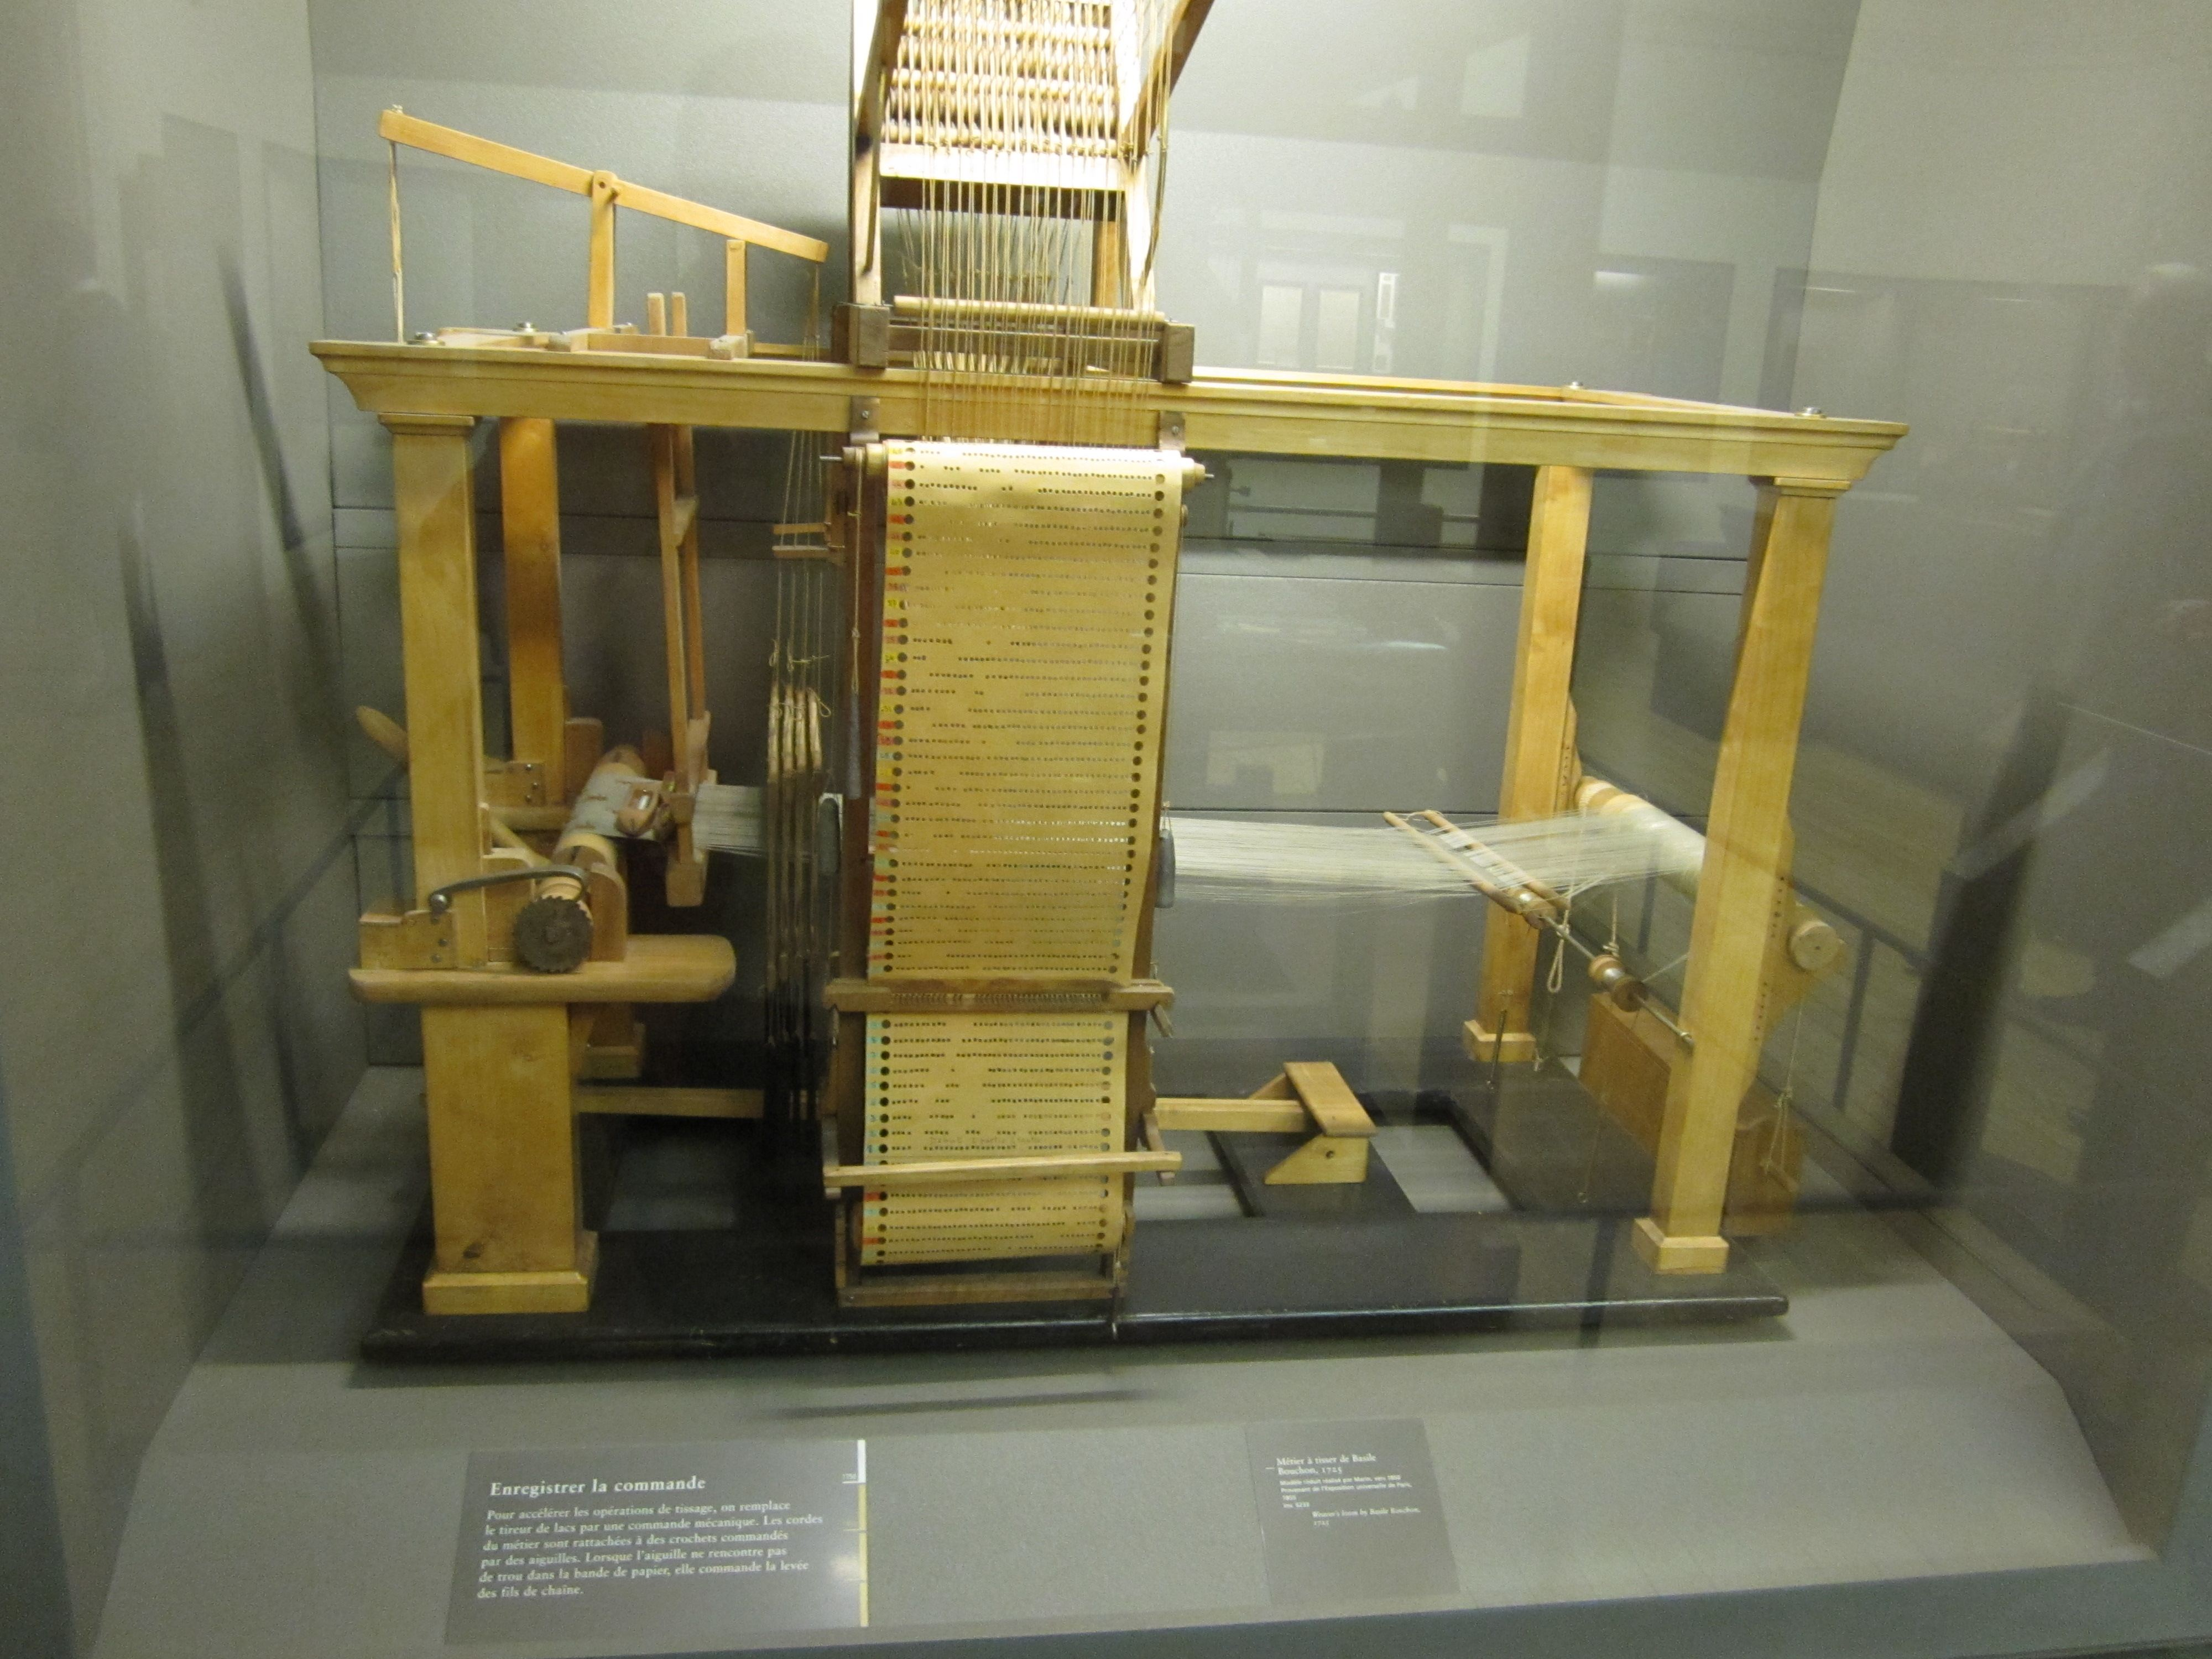
\includegraphics[width=0.8\textwidth] {bilder/bouchonloom.jpg}
\caption{A Bouchon loom exhibited at the Musée des arts et métiers in Paris.}
\end{figure}
% Bild på xerox-musen eller mac-musen
\nocite{bouchonloom}


\subsection{Herman Hollerith and the Census Problem}
By the end of the 19th century the Bureau of the Census in the United States were having a problem. The Census is the agency in charge of keeping records of the population, and due to heavy immigration, the amount of data and complexity of the system was rapidly increasing. At that time, the Census was performing a population count every ten years - a process taking years to complete. In 1889, the director of the Census advertised a competition for the 1890 census tabulation system. The competition involved tabulating the St. Louis population district information from the previous 1880 census. The winner of the competition was Herman Hollerith, a former employee of the census bureau, with his electric tabulating machine.\cite{aspray1990ch4}

\begin{figure}[h!]
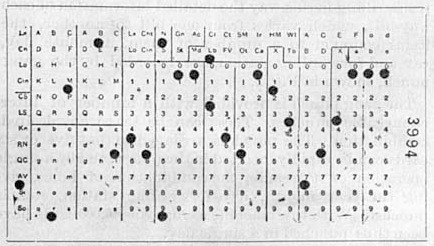
\includegraphics[width=0.8\textwidth] {bilder/punchedcard.jpg}
\caption{A punched card used in the 1890 Census, published in the Railroad Gazette 1895.}
\end{figure}
% Bild på xerox-musen eller mac-musen
\nocite{punchcard}

[short description of the machine].

Hollerith's tabulating machine was a success, and the contract was renewed also for the 1900 census. In order to expand the custormer base for his tabulating machines, Hollerith founded the Tabulating Machine Company in 1896. His company was one of three companies that in 1911 merged to form the Computing Tabulating Recording Company (CTR) - later renamed IBM\cite{IBMhistory}.

[short description of later date machines]

Punched cards were the most commonly used data medium until the 1950s, and were commonly used until the mid 1980s when they had become obsolete by the \emph{computer terminal}.

\subsection{The Teleprinter and the Terminal}
In 1901, Donald Murray developed a \emph{tele-typewriter} or \emph{teleprinter}. His idea was to simplify the work of telegraph operators, by using a typewriter keyboard. The operator would type on a typewriter, where every letter corresponded to a pattern of holes punched into a punch card. The information on the punch card was then transfered over the already existing telegraph lines and reproduced at the receiving end, again on punch cards.[citation needed] PROBABLY: WORLD's WORK

This method of typing to punch cards was used by the first computers, and are known as \emph{computer terminals}. The term computer terminal is not exclusive to punch card-based typewriters. Though punch cards were the main method of data entry and data storage, alternative methods began to emerge in the early 1960's. 

In the 1960's, output devices had become more advanced and in the end of the 1960's, the first attempts were made to replace printing with a \emph{computer monitor}. This method of combining a typewriter-style \emph{keyboard} with a monitor is known as a \emph{computer terminal}. One of the earliest computer terminals was the Datapoint 3300 by the Computer Terminal Corporation\cite{datapoint}. Using the Datapoint 3300, the user could control a \emph{cursor} by moving it up, down, left and right on the screen, but the terminal had no microprocessor.

Microprocessor computers allowed the combination of program and working memory and it allowed the computer programs to read data from the memory itself. To input data into the memory, punch cards could still be used. However, since all the data was stored electronically the data could as well be entered direcly into the memory. This removed the need for the punched paper middle step. The data that was previously transmitted via telegraph lines could be used to connect the typewriter directly to the computer memory. The initial disadvantage with this method was that memory was limited and expensive. Thus, the use of punch cards declined in favour of the computer terminal, in step with computer displays becoming more available\cite{aspray1990ch4}.

\subsection{Pointing devices}
The first computer \emph{mouse} was developed in 1965 at the Stanford Research Laboratory and is contributed to Doug Engelbart. Engelbart also proposed applications for the mouse, such as using multiple tiled \emph{windows}, which became widely used in early graphical computer interfaces. Although invented in the 1960's, it was not commercially available until 1981 when released as part of the Xerox Star system\cite{myers1998bhh}. Xerox soon got competition by the Apple Lisa (1983) and the popular Apple 128K (1984).

\begin{figure}[h!]
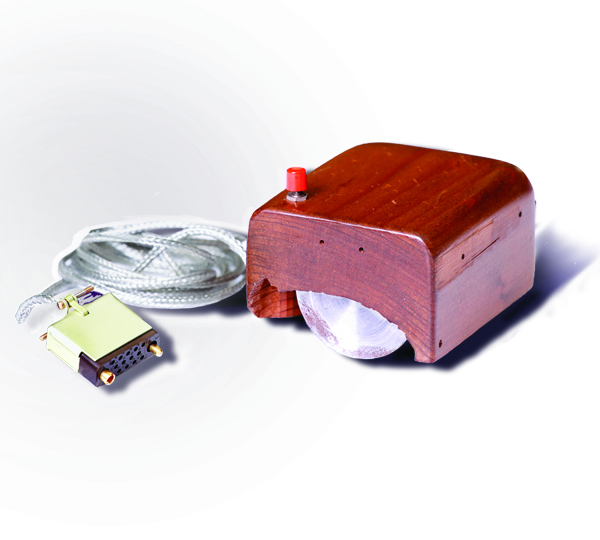
\includegraphics[width=0.8\textwidth] {bilder/firstmouse.jpg}
\caption{The first mouse prototype by Engelbart 1865.}
\end{figure}
% Bild på xerox-musen eller mac-musen
\nocite{srimouse}

\begin{figure}[h!]
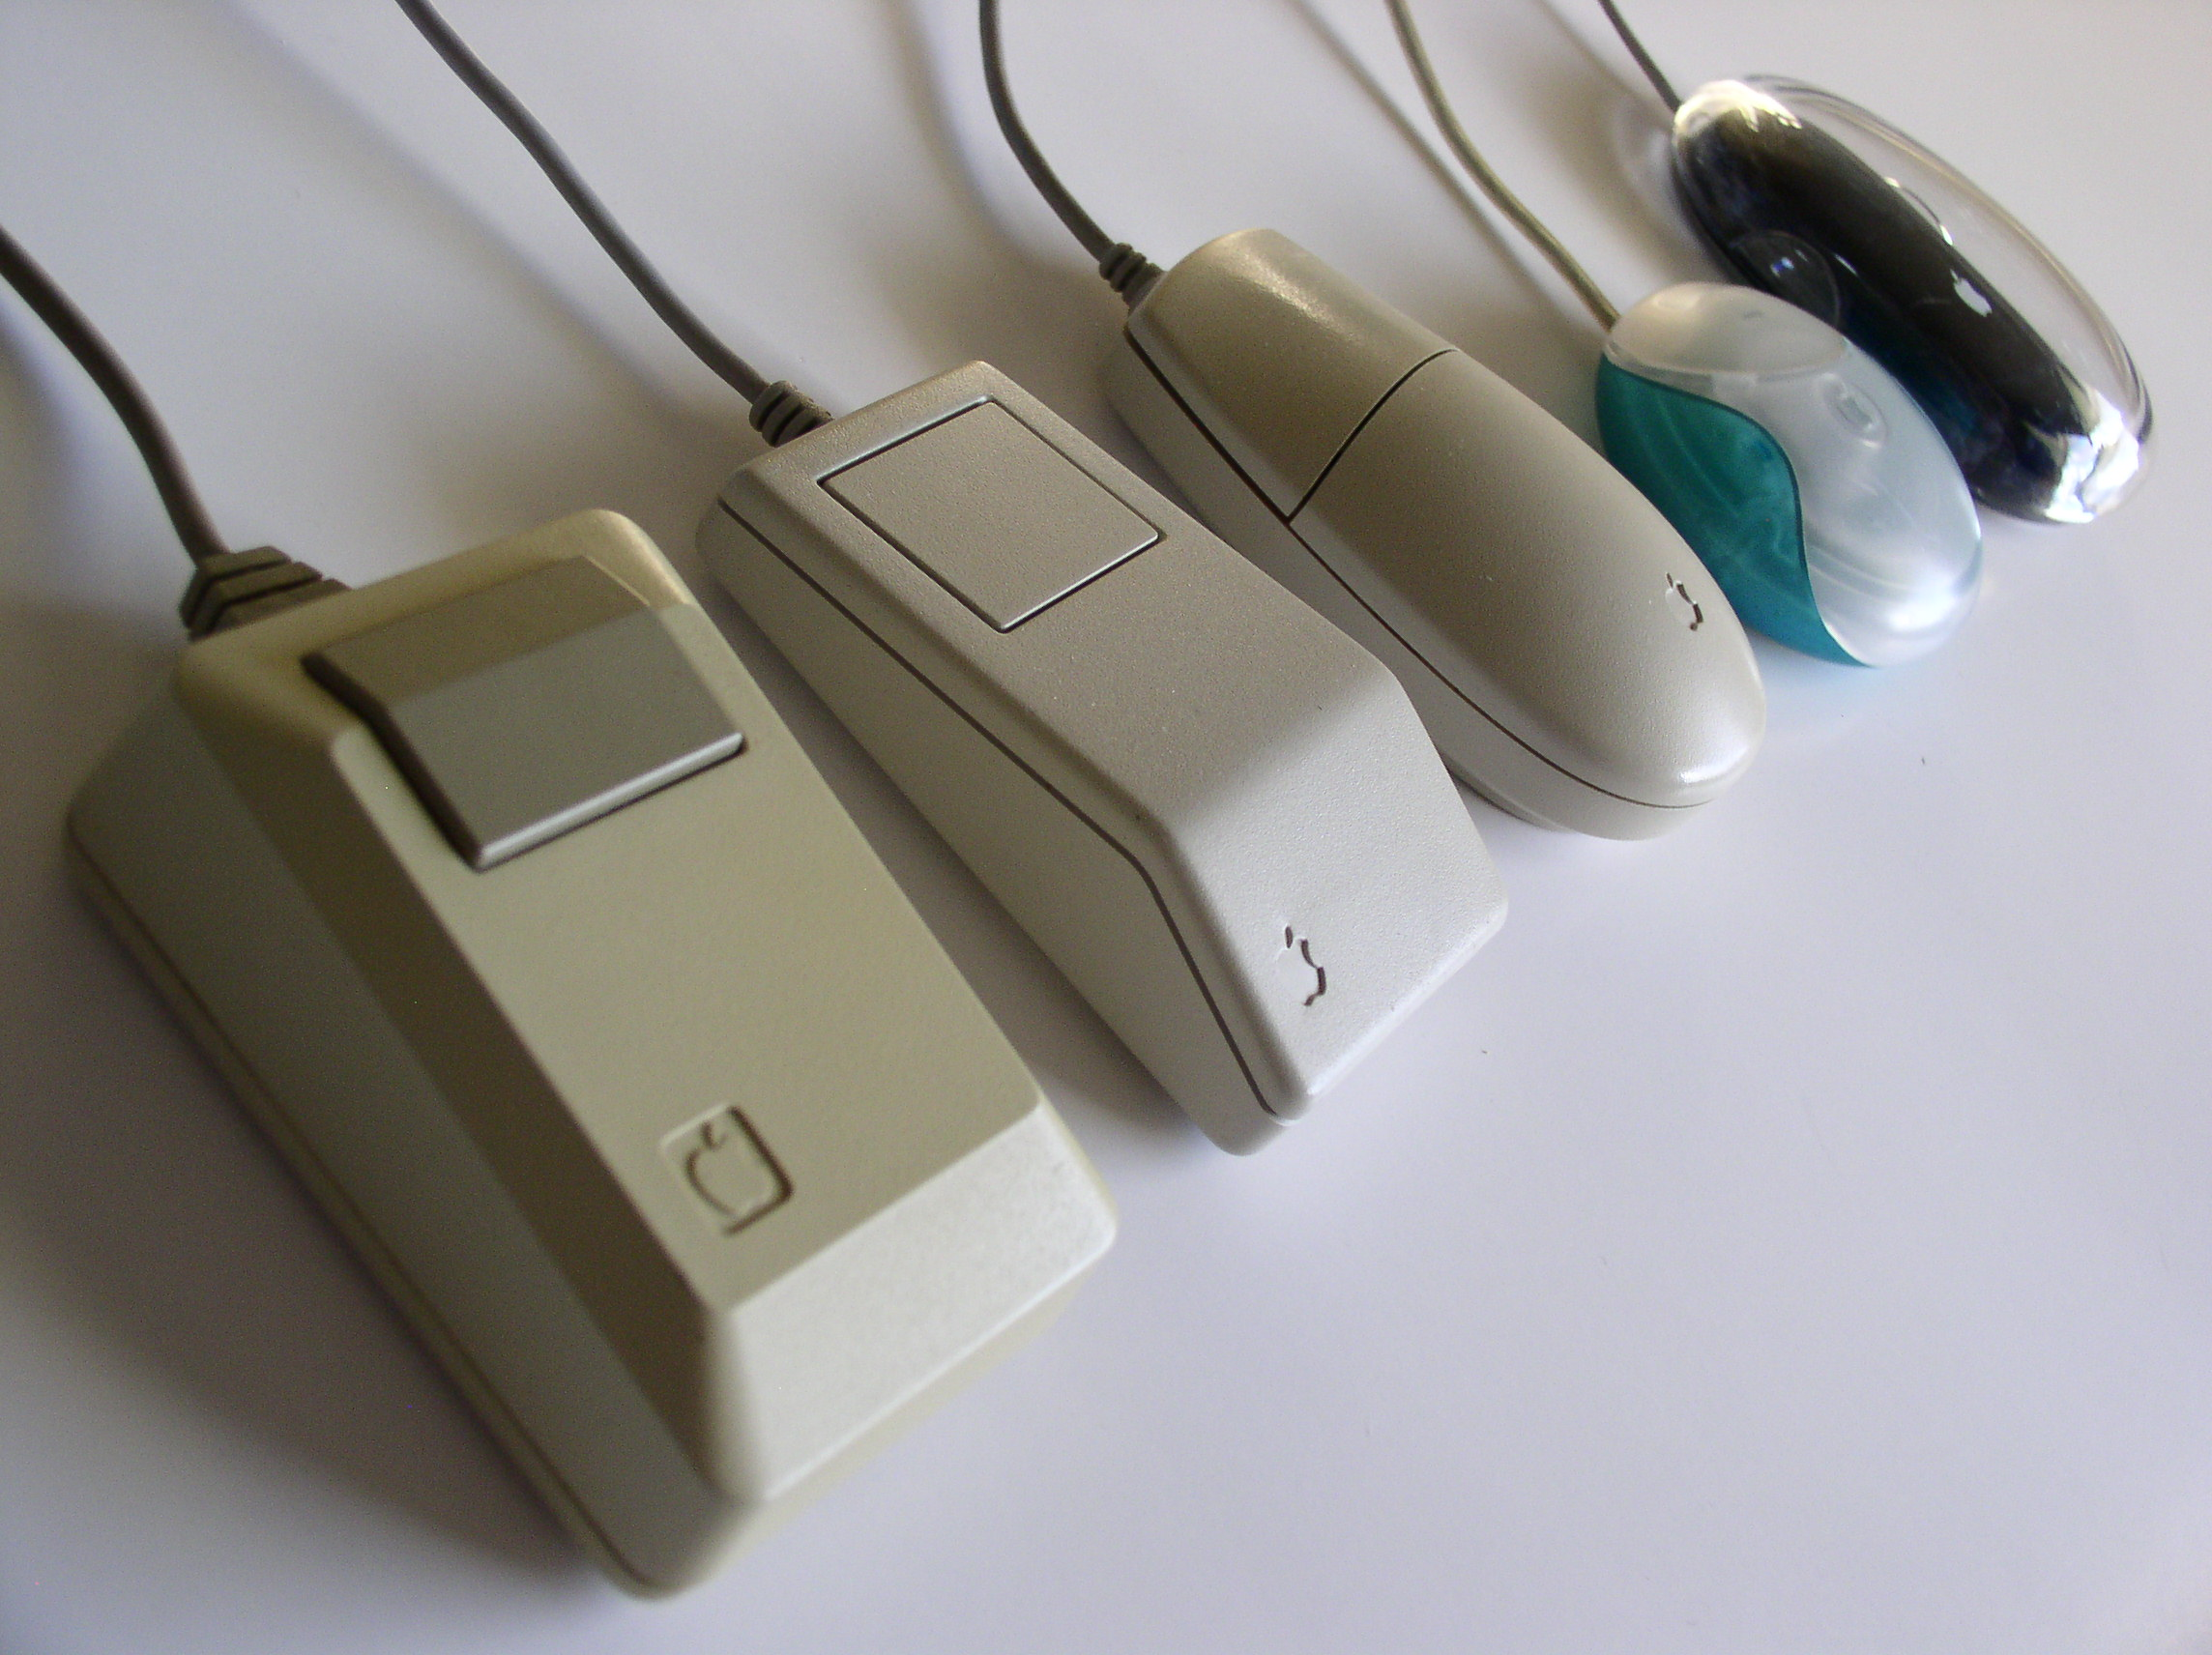
\includegraphics[width=0.8\textwidth] {bilder/applemice.jpg}
\caption{A series of mice from the Apple company from different era. The Apple 128K was supplied with the Macintosh mouse (closest in the picture).}
\end{figure}
% Bild på xerox-musen eller mac-musen
\nocite{applemice}

The introduction of this device allowed the users to move a pointer on the display that could be used to interact with the computer. A ball underneath the mouse gave relative x and y coordinates when rolling the ball on a surface. The mouse laid the ground for the WIMP (Windows, Icon, Menus, Pointer) graphical interfaces used today\cite{journals/cacm/Dam97}. The graphical user interface was invented by XEROX, and the Star system is wildely recognised as the first commercially available product with a graphical interface.

%As the displays became smaller and smaller and with the introduction of flat screens the portable computers were introduced. To keep these computers portable the mouse had to be built into the computer itself. This lead to a different kind of pointing devices.

%The portable computer pointing device problem was initially solved by turning the mouse upside down and using a "pointing ball" (pointing ballen kan ha kommit tidigare).

%The pointing balls were cumbersome/too large/nånting and a new input method for portable computers were needed. 

%Jag vet ingenting om styrplattor. 





% !TEX root = rapport.tex
\section{Current}
% Kolla upp hur utgågna patent på current devices spelar in, det verkar vara en faktor på åtminstånde touch screen, kan säkert vara intressant på voice också.
% Brasklapp
% Fundamentals: Asmycket referenser i kapitel 1.4


Several input devices in this paper such as the keyboard and the mouse, are still wildely used but can be seen as historical devices. This is justified by the fact that they remain largely unchainged - if not in their physical design then in the fashion they are used [©itation needed]. On the other hand, a number of other input/output devices that can be seen as to be recent have a long history behind them. taken a larger and larger market share. Although \emph{touchpads}, \emph{touchscreens} and \emph{speak recognition} techniques were researched as far back as the 1960's \cite{buxton}\cite{shoebox}, they have only now began to see commercial use and have likely still not reached their "peak". 


\subsection{Touch devices}
Touchscreen devices have become increasingly popular during the last years, through the breakthrough of \emph{smart devices} (i.e. smart phones and tablets) running specialized operating systems such as the Apple's iOS and Google's Android. The technology used in these devices however, have evolved over over a much longer time.

One of the first mentions of touchscreens was by E.A. Johnson in 1965, describing a touchscreen and identifying some potential uses in a short article, less than a single page\cite{4205802}. Some of the earliest developed systems came in the beginning of the 1970's. Early prototypes are the PLATO IV\cite{buxton} (1972) (seen in figure \ref[platoIV] and a transparant touchscreen was developed and put to use by CERN in 1973\cite{cern}.

% http://cooper.library.uiuc.edu/archives/archon/?p=digitallibrary/digitalcontent&id=1478
% NOTE: USE OF THIS PICTURE HAS NOT BEEN APPROVED. I'VE EMAILED THE UNIVERSITY
% OF ILLINOIS, AND I'M AWAITING REPLY.
\begin{figure}[]
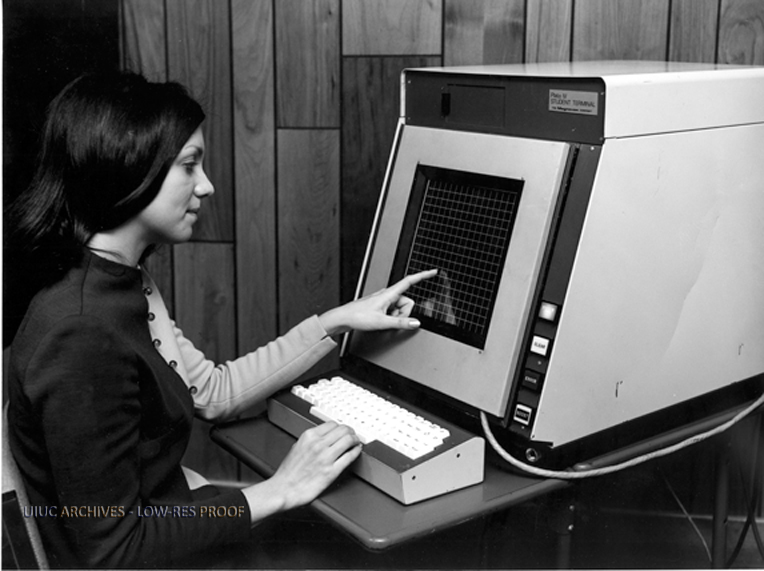
\includegraphics[width=0.8\textwidth] {bilder/platoiv.jpg}
\caption{Student using the PLATO IV.}
\label{platoIV}
\end{figure}
% Bild på xerox-musen eller mac-musen
%\nocite{platoiv}

%These devices used METOD - PROBLEM MED DETTA - BESKRIVA NÄSTA GENERATION. (DET SKA HANDLA OM LJUS HÄR, JAG REFERERAR TILL DETTA OSKRIVNA STYCKE SENARE.

The initial uses of touchscreens were point-to-select systems used in for example ATM machines or cash registers in restaurants and were relatively non-demanding on the screen performance\cite{buxton}. But there were also early attemps to make \emph{PDAs}\footnote{Personal Digital Assistant}. The first products to enter the market were the Palm Zoomer and the IBM Simon. The Simon was a mobile phone without any physical buttons, having only a touchscreen as its working area. But beyond regular telephone capabilities, it could also manage information such as a telephone book and be used for drawing and taking notes. Due to this, it is sometimes refered to as the first \emph{smartphone}\cite{buxton}.

Smartphones have seen much development since the release of Simon, and today (2013) it is estimated that more than a billion people use smartphones\cite{billion1}\cite{billion2}. [KORT STYCKE MED REFERENS SOM SÄGER ATT DET ÄR PGA ANDROID OCH IOS]. 

This increase in the number of touch-based devices has changed the way in which we interact with computers. New operating systems especially designed for smartphones and other smart devices, such as the popular IOs and Android operating systems have a fundamentally different approach to computer interaction.

The traditional WIMP approach requires the user to find the cursor on the display, move it to the desired location and click the mouse button to interact, or use the keyboard to input data. The touch screen on the other hand gives the user the ability to point directly at the desired item at the screen to activate it. An on-screen keyboard appears only when it is needed, allowed the computers to show only what is relevant at any point of time. This has made computers so portable that they can be used in almost any context and in a user friendly way [JAG TROR JAG KAN HITTA EN BRA REFERENS I MIN HCI-BOK]. The tablet is so simple in its design that it can be used by small kids and even cats [Bild på frasse tagen med en smartphone. Prata om att smart devices gör saker som att ta bilder].

%Multitouch. Vad är det, och varför?
One of the big breakthroughs that has allowed the touch screen to become the only input device required by a computer is the introduction of multi finger gestures. While touch screens previously only handled one action ("left mouse button"), the use of multi hand gestures removes the need for "icons" [DET FANNS ETT BRA ORD I NÅN ARTIKEL, HITTA!]. The rest of the functionality can be reached by for example pinching or swiping one's fingers. This type of interaction is not fundamentally more user-friendly, but it can be if used in the right way.

\begin{figure}[]
\includegraphics[width=0.8\textwidth] {bilder/ipadbook.jpg}
\caption{Apple Ipad showing iBooks, with the book Alice's Adventures in Wonderland.}
\label{ibooks}
\end{figure}
% Bild på xerox-musen eller mac-musen
\nocite{ipadbook}

Consider the common act of reading an e-book on a tablet. On a traditional computer, one typically reads the e-book as a document, with all pages following each other from top to bottom. On the tablet, the e-book can be made to look like a book, see figure \ref{ibooks}. The act of swiping one's finger from right to left triggers the book to turn the page, similar to what one would do in a physical book. This could be done with another gesture, for example by drawing a circle on the screen or triple-tapping an so on, but these approaches would not at all be as intuitive as the swipe-gesture.


\subsection{Voice recognition}

Voice recognition is another input method that has become increasingly popular during the last years. This input method uses speech recognition by analyzing input from a microphone. One the spoke word has been analysed, it can be used in several ways.

One ambition is that of providing real-time subtitles to spoken text, for example to aid those with hearing disorders. As an input method, the sound input can be parsed by the computer and then trigger a predefined action. In the past year (2012???????), Microsoft presented an English to synthesised speech Chinese translator, working in real time[CITATION NEEDED]. 

\subsection{Typ en egen subsection}

While the computers have become powerful and cheap enough to make speech recognition broadly available recently, its history is much longer. The first working implementation was introduced by Bell Labs in 1952. The system was able to recognise spoken language at telephone quality, and had a success rate of between 97-99% [REFRENS TILL DAVIS, JAS000637.pdf].

Early speech recognition attemps were simple, and could not analyse sentences. Instead, single words were compared to a rather small dictionary, compared to those used today. The Bell Labs system from 1952 was able to recognise the numbers 0 to 9, spoken by a single speaker.[citation B.H. Juang - Automatic Speech Recognition – A Brief History of the Technology Development] The user was forced to make a small pause between every word for the system to recognize them. 

Another system worked by analysing phonems in the spoken text. Phonemes are the smallest building blocks of the language and consist of the individual sounds used to construct words and sentences[REFERENS TILL KOG.PSYK-boken]. Early phonem-based techniques could only recognise a subset of phonemes. RCA Labs in 1956 could recognise 10 phonemes, spoken by a single speaker. Fry and Denes at the University College in England could recognise 4 wovels and 9 consonants. More notably, they were the first to incorporate statistical information in the analysis[Juang] - something that now is fundamental in speech recognition. By analyzing speech at this low level the system becomes less dependant on pauses and dialect in speech.

In the 1980's, the use of \emph{Hidden Markov Models} was introduced in speech recognition[REFERENS HMM.pdf]. Hidden Markov models are statistical Markov models where the path through the process is not observable. The Markov Models use previously gathered statistical data to with some certainty guess which phoneme the user is saying, and the chain of phonemes considered to be correct are then matched to a phoneme-word database to decide which word the user has spoken. The context of the word is also taken into acount to prevent homonyms of the desired word to be entered instead. The Markov Model Speech Recognition systems "learn" the users voice and speech patterns by using the data from corrections to alter the statistics used to decide which phoneme was spoken. 

This next part will explain what markow chain thingies are, with a reference to the picture.

\begin{figure}[]
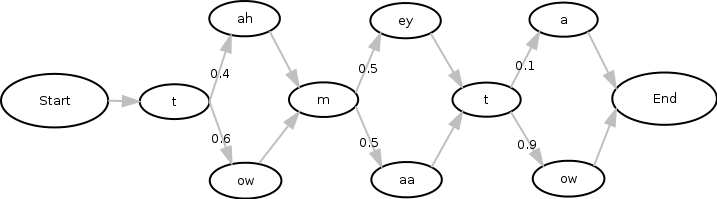
\includegraphics[width=0.8\textwidth] {bilder/tomato.jpg}
\caption{A model describing the statistical values of phoneme input of the word Tomato. The model contains american and british english pronounciations, with a small statistical favor of the british accent.}
\label{ibooks}
\end{figure}

Most speech recognition software today use Hidden Markov Chains for speech analysis[ÅLANDS REFERENS], but recent research has shifted focus towards the user of a type of artificial neural network, called Deep Neural Networks (DNN). Neural networks have been used for speech recognition since the late 80's, but the use of DNN is the first that has been shown to have substantial benefits over the use of the traditional markov chain approach. A research collaboration around DNN exists between the University of Toronto, Microsoft, IBM and Google. Late 2012, Microsoft publicly demonstrated their work with speech recognition - a system that can translate spoken English into spoken Mandarin in real time and in the voice of the speaker. In conjunction with the demonstration, Microsofts chief researcher Rick Rashid says about DNNs: "While still far from perfect, this is the most dramatic change in accuracy since the introduction of hidden Markov modeling in 1979". [Ref:http://news.cnet.com/8301-10805\_3-57547627-75/microsofts-new-translation-tech-speaks-chinese-in-your-own-voice/]

In the 1990:s personal computers became fast enough to power speech recognition software. 


Referens BLABLA:
A. Waibel, T. Hanazawa, G. Hinton, K. Shikano, and K. J. Lang, (1989) "Phoneme recognition using time-delay neural networks," IEEE Transactions on Acoustics, Speech and Signal Processing, vol. 37, pp. 328-339.

\subsection{Discussion}

% en diskussion och analys som sammanfattar båda ovanstående kategorier.
\section{Future}

\section{Special-Purpose Devices}

Computers today are used for the most diverse set of tasks. They have become such an integral part of our society that persons with handicaps that prevent them from using computers are at risk of getting left out of large parts of society and from work opportunities. While the computers themselves are indifferent towards handicaps, the input and output devices present the user with accessibility problems.

The obstacles for people with impaired vision are mostly concerned with output devices, since most output devices rely on graphics like bitmap displays or status LEDs. This can be circumvented with accessibility tools, such as the Apple Inc VoiceOver solution described below. But input methods may also present problems, for example the touchpads used in modern mobile phones.

For people with reduced motor skills, the obstacles lie mainly in the use of input devices and come in many different degrees. The standard computer mouse  can for too sensitive for some users, whereas both the mouse and keyboard may be unusable. Below, some of the most prominently used special-purpose devices are described.

\subsection{Alternative Input Methods}
Devices aimed towards aiding people with reduced motor skills come in different types, depending on which issue they are designed to conquer. In some cases the use of hand controlled devices is a problem, which has generated much research on \emph{foot-controlled devices}. AUTHORS describe SOME PRODUCT that DOES SOMETHING WITH THE FEET. MORE INFORMATION.

%Bild som beskriver detta

Another set of devices are designed to aid persons that have lost most all of their motor skills. AUTHORS describe devices that are controlled using eyes or facial features that do not require any other movement. These devices are called \emph{gaze communication devices}. Devices that use gaze communication, as described by AUTHORS, MULTIPLE\_REFERENCES are designed to allow persons who have extensive motor skill handicaps to use a specialised pointing device for controlling the computer. These devices rely on facial features and actions for controlling the cursor on the display, like nose tip and pupil movements for cursor movements and blinking for performing click actions.

%Bild som beskriver detta

AUTHORS REFERENCE describe a special-purpose input method, designed mainly for smart phones and tablets which use touch screens, to input text using \emph{Input Finger Detection} (IFD). Most smart devices today have some kind of input method to aid blind users or users with impaired vision. The VoiceOver solution from Apple reads the selected virtual key out loud. The user then selects it by double tapping on the display[citation needed, apples officiella].

[Beskriv att det som följer är en case study typ]

A special purpose device that allows the user to enter text in a much faster pace when handling touch screen devices, in comparison to VoiceOver is the Perkinput method[citation needed]. The method allows the user to enter \emph{Braille}[Fotnot needed, short explanation of Braille] letters directly by tapping fingers on the display.

The Braille alphabet is built using a 2x3 \emph{bit[fotnot, similar to but different from computer bits] matrix} where each letter has certain \emph{bits} "up" or "down" [reference to figure]. In the Perkinput system, using two hand Braille input the user taps up to six fingers on the display - each finger representing a bit in the Braille letters. The letters can also be entered using only one hand by first entering the left column with three fingers, followed by the right column with the same fingers.

For entering letters using two hands, the user uses three fingers on each hand. Each finger represents one of the bits in the Braille letter. To enter the letter B, having binary representation 110000 using two hands, the user would press the first two fingers on the first hand only, representing only the first two bits as 1:s.

To enter the letter B, using one hand, the user would press the two first fingers to represent 110, and then do a one finger swipe to represent the remaining 000.

The input rate of this special-purpose method is according to AUTHORS one handed Perkinput is evidentially faster than the iPhones standard input method, and two handed Perkinput is more than twice as fast. This comparison shows the difference a special-purpose device can make in the effectiveness of computer use related to adapted standard input methods. 

\begin{figure}[h!]

	\centering

\begin{tabular}{c c c}

$
\begin{array}{cc}
\bullet & \circ \\
\bullet & \circ \\
\circ & \circ \end{array}
$

&

$
\left[ \begin{array}{cc}
1 & 0 \\
1 & 0 \\
0 & 0 \end{array} \right]
$ 

&

110000 \\

(a) & (b) & (c)

\end{tabular}


	\caption{Three representations of the Braille letter B; the regular representation (a), a matrix representation (b), and a binary representation (c).}

\end{figure}

\subsection{Discussion}
The input devices are much more diverse in their designs, because they need to adress a larger set of handicaps. The output devices mainly focus on sight, and somewhat on hearing (visual alerts -- hitta referens), while input devices are needed for a whole spectrum of handicaps. Two main categories of special-purpose input methods are devices to aid persons with reduced motor skills, and persons with reduced or no eye-sight. 

Prata om att inte alla lösningar är hårdvarubaserade, referera till case studyn.


% !TEX root = rapport.tex

\todo{Braille är ett egennamn (Louis Braille) och ska skrivas med stor bokstav, det måste vi kolla innan inlämning.}

\section{Results}

%history:

The earliest computer interaction devices were not initially designed for computers nor to make computers user-friendly. Instead previously existing technologies were directly taken and modified in order to function within their new setting. In contrast, the computer input devices in use at the time of this study are designed to make human interaction with computers as simple and easy as possible.

The typewriter-based \emph{terminal} was in a way the first input device specifically designed for computers. It removed many of the earlier problems associated with programming and running calculations on the computers of that time. Although this device was very different from the earlier input devices, the underlying technology was still based on the previous input systems, punch cards, although it abstracted away technicalities that slowed the user down. In contrast, the development of pointing devices was not related to the previous systems, but instead a result of the introduction of bitmap displays, capable of displaying data in a different way than previous computer displays.

The big difference between these important inventions is the type of impact they had. The terminal allowed the user to communicate with the computer more conveniently than before, but still in the same style. The mouse instead changed computer usage altogether, being instrumental in the window-based systems introduced in the 80's. The impact of touchscreens is in a way similar to that of the mouse, in that it has lead to a new type of graphical user interfaces. Importantly, as these systems are mostly mobile devices, it has not only changed the way we use the computer but also how and when we can use them.


%Här är ett stycke som wrappar ihop de fyra tidigare. Den säger att fokus blivit mer och mer på användarvänligheten, och att de hör ihop. Man lärde sig att skiva text smidigt, men ville kunna lätt byta mellan olika "fönster" och flytta pekarens plats lättare. Touchpad, för att musen var för klumpig på laptop, touchscreen för att kunna ha bättre kontroll eller whatever. Jag vet inte riktigt varför man ville ha skiten, men vi skriver något.

%ny text (14/5):

There has been an apparent change in the focus of computer input devices from machine centric input methods in which the user has to adapt to the technical limitations of the first computers to a clear user centric approach. While the pointing devices were developed to handle input to the new graphical output methods and not specifically to ease the overall computer experience, the effect on user friendliness are apparent. This laid the ground to the creation of computer interfaces that were more accessible to users without technical background and allowed the computers to move into the homes and offices of regular citizens. This mass market opportunity created the necessary foundation for focus on more human centric computer interfaces that we are still feeling the effects of today.

%current:

The two current input methods discussed in this paper, speech recognition and touchscreens, behave very differently in practice, but they share the same underlying idea - to remove the hurdles in the interaction between man and machine. The touch screen has evolved as the next step from computer-mouse-keyboard interaction to direct interaction with the data the user is interested in. This allows the user to manipulate the data using fingers and the learning curve for users is drastically reduced when the computer interacts with the user in the same way a physical object would do.

Speech recognition fulfills the same goal in easing the interraction between human and computer, but instead of doing it physically it is done by reacting to the spoken language in the same way the user would speak to another human. The idea is to make the computer understand the user on the user's own terms. The development of speech recognition systems has required research in cognitive psychology and mathematic (statistical) models rather than on computer science, which reflects the previously mentioned change of focus towards user-friendliness.[reference?] \todo{reference? behövs det i results-delen?}

%special:

Computer interaction for people with different kinds of handicaps are often dependent on special purpose devices, depending on the nature of the disability. As computer output most commonly use displays, they only pose a problem for users with low eyesight or blindness, and the existing solutions are either tactile or hearing-based. The input devices on the other hand are much more diverse in their designs, as they need to adress a larger set of disabilities. Two main categories of special-purpose input methods are devices to aid people with reduced motor skills, and people with reduced or no eye-sight. Additionally, for persons with reduced motor skills, there are different methods available depending on how much motor skills is assumed.

%Hur bra är alternativen? Kan de ta del av viktig information i sin vardag? Hur hög medvetenhet finns det generellt? (tänker en webdesigner på sån nuförtiden?)

For a person that has reduced motor skills in the hands only, the use of the standard keyboard and mouse can be difficult or impossible. There are solutions where a special designed keyboard and mouse designed for use with the feet can overcome this problem.
For persons that have more extensive reduction of motor skills the use of such devices might also be a problem. There are numerous different approaches to solve this. One of the most interesting is the use of eye movements to steer the computer. This approach makes use of cameras to track the users eye movements and act as a pointing device, which is also used to control an on-screen keyboard. 

For persons that have reduced eye sight the use of Braille input can be used to overcome computer use problems. There are numerous approaches with redesigned standard equipment like Braille keyboards, and speech feedback. There are also some completely different approaches that are more user centric, as an example the Perkinput system that uses the fingers on a touch surface (touch screen) to input Braille characters.

As illustrated by the case study of the Perkinput system, not all special purpose devices rely on specially designed hardware, but may rely on the software that handles these input devices. The Perkinput system allows the user to use the standard interface of the smart phone or tablet, but use a fundamentally different method of inputing text that is handled by the software that ease the process of data input into the system.

% ett stycke som binder samman special och future

% future

%ny text (14/5):

The future devices discussed in this paper, gesture input and brain-computer interfaces are taking an even larger step away from previous computer input devices, in that they completely remove the computer as an entity in our workflow. Instead they let us focus on the task at hand without even reflecting about that there is actually a computer doing all the work in the background. This will allow the introduction of computer assisted processes in completely new parts of human lives. \todo{skriv om case study av bil-grejen.}

\section{Discussion}

% både tangentbordet och musen kom tidsbesparingskäl, istället för hålla på med hålremsor eller försöka styra grafisk information med tangenter.

Computers have gone from being big black boxes that take specially formated input and produce computer formated output that has to be interpreted by a human, to become more and more seamlessly integrated with regular human life. It has also evolved from complex systems that require professional training to seemingly simple devices usable by even small children. In this transformation a few trends can be observed. The first is the process of making computer input faster while still retaining the underlying structures, the second is to make computers available to larger groups of people by making them simpler to use, and the third is the process of removing the computer as an entity and making it transparent to the user.

The first trend had no intentions to change the nature of computers at all, and did not do so in any extensive way. The introduction of keyboards and terminals were simply a way to speed up the process of computer input/output and were mostly technology driven. 

The second trend, of making computers accessible to larger groups of people, set in motion a large scale research and development cycle in both academic and commercial sectors which changed the focus from large main frame computers to desktop computers which introduced the user centric approach to computers.

The current state of human computer interfaces display an even larger focus on making the computers transparent to the users.

Since the aspect of making computer systems human centric was introduced many different input devices have been introduced and are being used for tasks that were previously performed at a terminal type computer. However, these systems do not necessarily replace the previous computer systems, instead the spectrum of computer interfaces in use is broadening. The concurrent use of different kinds of interfaces means that each individual interface is becoming more and more adapted to its context of use. The act of typing moderate or long pieces of text is tiring on a touchscreen device, being too slow and lacking the physical feedback of a real keyboard. On the other hand, inputing small amounts of data on the go is an activity that is only made more cumbersome by a physical keyboard and benefits heavily from the compact form of a touch screen device.

Examples of this concept can be seen across the field, where desktop and laptop computers are being replaced in areas were newer technology is more suited, while they still remain in areas were newer input systems have yet to outperform the previous setup. It is also evident that some of the current systems are outperforming each other in different areas. An example is that the use of voice recognition has become more and more used in simple query based tasks, with technologies like Apple Inc's Siri voice recognition system, where touch screen based systems in smart phones were previously prominent.

With the mainstream systems getting more and more diverse the division between special purpose devices for persons with disabilities and standard devices will probably become less and less important, since every device will have different designs and ways of accessing the data. As this process continues these devices will become just another device in the myriad of devices available. \todo{rimligt?}

In summary, computers have gone from a single technology centric design with a unified interface, to a large number of context specific interfaces designed for more and more diverse tasks. With the context specific interfaces the computers themselves become such an integrated part of the process they are part of that they become invisible to the user. It is highly likely that this trend will continue and that we will see custom designed computer interfaces in almost every aspect of our lives. This will likely reduce the terminal type computer, which has dominated the market for over 40 years, from an all-purpose system to the typewriter on which it is based. The gap created will be filled by more suited and transparent devices more adapted to perform the current and future tasks we will use computers for.

\section{Proposed Future Work}

\todo{write me!}

\bibliographystyle{plain} 
\bibliography{references}

\end{document}
